\documentclass[14pt]{article}
\usepackage[margin=0.8in]{geometry}
\usepackage{fancyvrb}
\usepackage{graphicx}
\usepackage{subcaption}
\usepackage{hyperref}
\hypersetup{
	colorlinks=true, %set true if you want colored links
	linkcolor=black, %choose some color if you want links to stand out
	urlcolor=blue
}
\graphicspath{ {./images/} }

\setlength{\parindent}{0pt}

\title{CCTF - Report}
\date{18/11/2020}
\author{Nail Dupre, Guadagnini Giovanni, Enrico Micheli, Davide Piva}

\begin{document}
	
\maketitle
	
\tableofcontents
\newpage
\section{Overview}
This report concern the two cctf laboratories:
\begin{itemize}
	\item \textbf{Resilient CCTF}: During this ctf the main purposes were both to attack and defend a HTTP server against different type of attacks.
	\item \textbf{Secure CCTF}: During this ctf the main purposes were both to attack and defend a small php webapp.
\end{itemize}

\section{Resilient Server}
As already introduced in the Overview section this cctf was targeted to both offend and defend an HTTP server. Each group during the experience have access to two Deterlab experiments, in the first experiment the group will act as defenders (Blue Team) and in the second as attackers (Red Team).

\begin{figure}[!h]
	\centering
	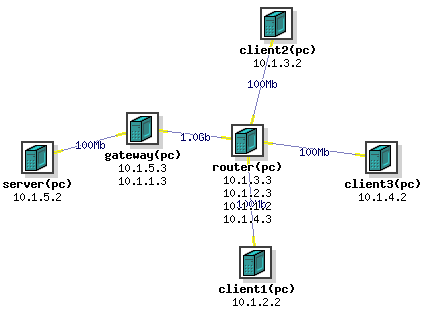
\includegraphics[width=8cm,height=6cm]{ResilientServerTopology}
	\caption{Topology of the Resilient Server CCTF.}
\end{figure}

This image describe the topology of the laboratory, that can be subdiveded in 3 areas:
\begin{itemize}
	\item \textbf{Clients machines}: These machines will be used from the attacker team. One of the three computer will be used as the genuine client that will try to reach the server with legitimate requests with a maximium rate of 1 request every second, the attackers will use the other two machines to attack the server in order to try to deny service to the genuine client.
	
	\item \textbf{Server and Gateway}: This two machine will be used from the defender team, in the specific the server will be equipped with a webserver, that serve 10 html pages, and the gateway will be used to try to block eventual attacks.
	
	\item \textbf{Router}: This machine will connect all the machines controlled from the two groups and will be used to calculate the score.
\end{itemize}

\textbf{Attention}: The link between router and gateway is different from all the other links. In the specific the link provide 1 gb of bandwidth and allows all the client connected to the router to send the maximum amount of data allowed from the 100 mb links, and this is very suitable to launch flood attacks.
\\
\\
During the ctf attackers earn a points when a genuine request from the client take more than 0.5 seconds to be received, and on the contrary the point is given to the defenders group if the request is received from the client before half a second is passed. 

\subsection{Dupre}

\subsection{Guadagnini}
The work started working by developing some milestones: 
\begin{itemize}
	\item monitor\_server.sh: This script perform a really fast check of the server status. By sending ping and curl requests the user can easily understand if the server it's slowed down by some attacks.
	
	\item analyze\_traffic.sh: This script launches two python programs that by using tcpdump, thanks to system function of os python module, and finally by analyzing the collected traffic, will enable the user to know with precision how many packets have passed through the gateway and also which client are sending data. This script in the end wasn't used since another version af the same script that uses only python seemed to be a bit faster.
	
	\item flood.sh: This is a simple script that act as a wrapper for the flooder program that will enable the user to flood an ip by specifying less parameter than usual.
	
	\item slow\_loris.py: This script has been dowloaded it from its repository and in the first moment has only been modified to request for the pages provided from the server.
\end{itemize}

The initial part has been concluded by writing the startup.sh script for all the machines involved the cctf:
\begin{itemize}
	\item Blue part startup.sh: This script by using ssh will connect to the server and will automatically install the apache2 webserver, enable syn-cookies, create the pages in the /var/html/www folder, enable the slow-loris mitigation for apache2, setup the iptable rules and finally upload the milestone scripts in a shared folder /home/cctf. Also will configure the gateway by uploading the script and configuring the iptables rules.
	
	\item Red part startup.sh: Through ssh will install all the packages needed and will all upload the milestone scripts on a shared folder /home/cctf in all the client machines.
\end{itemize}

In all the scripts the interface has been inserted as a parameter thanks to a sort of subscript that using the ip address of the interface was able to return the name of the interface as a result.
\begin{Verbatim}
# Retrieve the name of the internal interface of the gateway machine
$(ip a | grep 10.1.5.3 | tail -c 5)
\end{Verbatim}

\subsubsection{Strategies}
Has also been developed the defense and attack strategy, that which over time have been modified according to the results obtained during the internal tests.

\paragraph{Defense strategy}
The first idea used was to limit the attack surface to a minimum and therefore to reduce it to a minimum and indispensable, so the iptables both on server and gateway have been used to try to block the unnecessary traffic. A white list approach has been used to allow only some kind of traffic to pass and finally reach the server, in the specific has been allowed:
\begin{itemize}
	\item All the traffic from loopback interface.
	\item All the traffic generated and directed to deterlab control network (192.168.0.0/16).
	\item All icmp traffic between gateway and server in the network 10.1.5.0/24.
	\item Icmp packet generated from the external network with a maximum rate of 1 ICMP packet per second.
	\item The fragmented packets have been blocked to avoid fragmented attacks.
	\item All the incoming http traffic on port 80, and obviously the outgoing traffic generated from the server.
\end{itemize}
Finally has been specified the DROP default policy for all the iptables chains in order to block all the traffic that won't match the rules. 
\\
Rules configured in the gateway:
\begin{Verbatim}
sudo iptables -F
sudo iptables -A INPUT -i lo -j ACCEPT
sudo iptables -A OUTPUT -o lo -j ACCEPT
sudo iptables -A INPUT -s 192.168.0.0/16 -j ACCEPT
sudo iptables -A OUTPUT -d 192.168.0.0/16 -j ACCEPT
sudo iptables -A FORWARD -f -j DROP
sudo iptables -A FORWARD -p tcp -d 10.1.5.2 -s 10.1.2.0/24,10.1.3.0/24,10.1.4.0/24 --dport 80 
	-m state --state NEW,ESTABLISHED -j ACCEPT
sudo iptables -A FORWARD -p tcp -s 10.1.5.2 -d 10.1.2.0/24,10.1.3.0/24,10.1.4.0/24 --sport 80 
	-m state --state ESTABLISHED -j ACCEPT
sudo iptables -A INPUT -f -j DROP
sudo iptables -A INPUT -p icmp --icmp-type echo-request -s 10.1.5.2 
	-i \$(ip a | grep 10.1.5.3 | tail -c 5) -j ACCEPT
sudo iptables -A OUTPUT -p icmp --icmp-type echo-reply 
	-o \$(ip a | grep 10.1.5.3 | tail -c 5) -d 10.1.5.2 -j ACCEPT
sudo iptables -A OUTPUT -p icmp --icmp-type echo-request -o $(ip a | grep 10.1.5.3 | tail -c 5) 
	-d 10.1.5.2 -j ACCEPT
sudo iptables -A INPUT -p icmp --icmp-type echo-reply -i $(ip a | grep 10.1.5.3 | tail -c 5) 
	-s 10.1.5.2 -j ACCEPT
sudo iptables -A OUTPUT -p tcp --dport 80 -d 10.1.5.2 -o $(ip a | grep 10.1.5.3 | tail -c 5) -j ACCEPT
sudo iptables -A INPUT -p tcp --sport 80 -s 10.1.5.2 -i $(ip a | grep 10.1.5.3 | tail -c 5) -j ACCEPT
sudo iptables -A INPUT -i $(ip a | grep 10.1.1.3 | tail -c 5) -d 10.1.1.3 
	-s 10.1.2.0/24,10.1.3.0/24,10.1.4.0/24 -p icmp --icmp-type echo-request 
		-m hashlimit --hashlimit-name icmp_gw --hashlimit-mode srcip 
			--hashlimit 1/second --hashlimit-burst 5 -j ACCEPT
sudo iptables -A OUTPUT -o $(ip a | grep 10.1.1.3 | tail -c 5) -s 10.1.1.3 
	-d 10.1.2.0/24,10.1.3.0/24,10.1.4.0/24 -p icmp --icmp-type echo-reply 
		-m hashlimit --hashlimit-name icmp_gw --hashlimit-mode srcip 
			--hashlimit 1/second --hashlimit-burst 5 -j ACCEPT
sudo iptables -A FORWARD -i $(ip a | grep 10.1.1.3 | tail -c 5) 
	-d 10.1.5.2 -s 10.1.2.0/24,10.1.3.0/24,10.1.4.0/24 -p icmp 
		-m hashlimit --hashlimit-name icmp_srv --hashlimit-mode srcip 
			--hashlimit 1/second --hashlimit-burst 5 --icmp-type echo-request -j ACCEPT
sudo iptables -A FORWARD -o $(ip a | grep 10.1.1.3 | tail -c 5) -s 10.1.5.2 
	-d 10.1.2.0/24,10.1.3.0/24,10.1.4.0/24 -p icmp 
		-m hashlimit --hashlimit-name icmp_srv --hashlimit-mode srcip 
			--hashlimit 1/second --hashlimit-burst 5 --icmp-type echo-reply -j ACCEPT
sudo iptables -P INPUT DROP
sudo iptables -P OUTPUT DROP
sudo iptables -P FORWARD DROP
\end{Verbatim}

To protect the server against slow DoS attacks, such as slow-loris, the libapache2-mod-qos has been enabled and configured, this module basically disables the keep-alive messages when the connections in the pool are running out in order to try to keep the service online and available.
\\
\\ 
Moreover, in an attempt to reduce problems related to malicious opening of connections with the web server, the apache timeout time has been reduced from 300 seconds to 1 second which for the purpose of this competition is sufficient to keep a connection active for the time used to assign a point.
\\
\\
\textbf{Snort} was also tried to improve defenses with some basic rules. By using the installation script present in the an older laboratory in the end Snort was installed in the gateway. Snort in particular can be very useful for thwarting some attacks but it is very harmful for flooding attacks as being single thread it does not scale very well when the number of requests rises significantly. So using Snort was very useful since was able to stop slow\_loris attack very easily but when a simple Syn flood attack was initiated, the performance collapsed causing significant delays in delivering the packets to the server and therefore to the genuine client. another problem with snort was the installation time, in fact before using the program it was necessary to wait for snort to compile and install on the system which took a long time. For the reasons outlined above snort was discarded and other techniques were sought and subsequently used.
\\
\\
As a result of the attacks tested, the security measures implemented were able to defend the server from slow dos attack thanks to the apache module but were vulnerable to flood attacks as a way to limit large amounts of traffic directed to the server had not yet been implemented.
\\
\\
From the beginning rate limiters used with Snort or iptables seemed not suitable since they were cutting off good and malicious traffic without distinction for a certain amount of time. The final idea for the defense was trying to inspect the traffic and search difference between genuine and malicious traffic, in order to let only packets that should be genuine through the gateway. Two very useful iptables option has been found and used to cut the malicious traffic. In the specific the two modules named named \textbf{match-hex} and \textbf{match-string} by inspecting the content of the packets were able to identify malicious packets. 
\\
So in the end the defense, in addition to some configurations made in the server, consisted of 2 steps:
\begin{itemize}
	\item Use tcpdump and Wireshark to collect data and search for differences or special pattern in the packets.
	\item Use the two iptables modules to cut the traffic identified as malicious during the previous step.
\end{itemize}

Despite the large traffic generated by flood attacks, iptables, with a limited number of rules used to filter incoming traffic, has always managed to maintain good performance and for this reason it has been used as the main part of the defense.

\paragraph{Attack strategy}
Defense and attack strategies were developed simultaneously, when a problem was solved a new attack that took advantage of more sophisticated methods was created and used to try to send the server out of service. This process of continuos modifications led to the modification of the attacks so that with each "iteration" each attack was better and in the specific each time the attack were modified in order that it had been more difficult to distinguish genuine from malicious traffic. 
\\
\\
In an attempt to optimize the score gained / lost during the attack phase, the following idea was formulated and used: if the attacks we were using weren't working or were partially working, there was no need to send the maximum requests possible and accordingly to this fact the genuine traffic could be lowered to the minimum or just simply reduced to lower the number of points opponents were earning. So following this idea the genuine\_client.sh script was modified to change on-demand the rate of the request sent by reading a file created in the same folder, the rate could be easily modified using the script change\_rate.sh that remotely throug ssh was able to modify the rate value saved on the file.
\\
\\
In order for the slow\_loris.py to be less recognizable, the request header has been redefined to be the same of curl and the content of the keep-alive requests has been randomized in order to be more difficult to detect and block. 
\\
\\
By observing the attacks has been suggested also to use scripts or packages that were able to modify the header fields in order to make the attack packes as indistinguishable as possible from genuine traffic, for example by putting the window at the same value that is used by curl 64240 and using modified headers as for the slow loris attack.
\\
\\
Finally has been discovered that while using flood attacks a single process wasn't able to generate very big amount of traffic, for example over 70000 packet per second. So accordingly to the available bandwidth of the link has been suggested to lower down the number of packets generated from a single process during flood attacks in order to make sure to take advantage of the available bandwidth with multiple processes that were concurrently generating a reasonable number of packets.

\subsubsection{Results Evaluation}
During the two cctfs by analyzing the traffic an by using the match module of iptables the defenses were able to cut a very big amount of malicious traffic. 
\\
\\
During the first cctf, before the laboratory crashed a very big portion of the attack traffic was blocked from the gateway and it seemed that the server was able to respond to genuine requests quickly.
\\
\\
Unfortunately in the second ctf the adversary team has been were very smart and managed to make the defenses to be ultra-protective. In fact, using fragmented genuine requests, which were blocked by default by the gateway, they managed to score many points as the requests to the server never arrived. One of the methods used to defend, in addition to blocking fragmented packets, was in fact to check that the DF (do not fragment) bit was not set to 1 in requests, this was typical in syn packets of flood attacks, but unfortunately it was also used from the other team to generate the genuine requests. Also by interspersing fragmented and non fragmanted genuine requests they managed to "protect" their attack as it seemed that the server was working correctly.

\begin{figure}[!h]
	\centering
	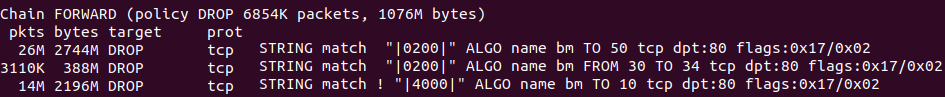
\includegraphics[width=20cm,height=1.5cm]{iptables_cctf_1}
	\caption{FORWARD iptables chain in gateway cctf1.}
\end{figure}

\begin{figure}[!h]
	\centering
	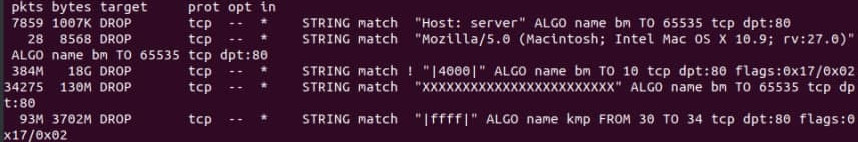
\includegraphics[width=20cm,height=3cm]{iptables_cctf_2}
	\caption{FORWARD iptables chain in gateway cctf2.}
\end{figure}
This images shows the rules added during the two cctf, as it's possible to see from the second column, the amount of dropped traffic is very big aroung 25 GB if we consider both the cctf. 
\\
In the specific the rules used were similar to the following:
\begin{Verbatim}
# Check for window = 65535
sudo iptables -I FORWARD 1 --match string --algo bm --from 30 --to 34 --hex-string '|ff ff|' 
-p tcp --dport 80 --syn --j DROP 

# Check for DF bit not setted typical of flooder
sudo iptables -I FORWARD 1 --match string --algo bm --to 10 ! --hex-string '|4000|' 
-p  tcp --dport 80 --syn --j DROP 

# Check for syn packet with malicious string in the playload
sudo iptables -I FORWARD 1 --match string --string "<malicious_content>" 
-p tcp --dport 80 --syn --j DROP
\end{Verbatim}

Has been really useful also the option "to" and "from" of the match iptables module since 
they could help narrow down which portion of the package to look for the pattern or malicious content.

\subsection{Micheli}

\subsection{Piva}




\end{document}
